\subsection{Synchronous Serial Communication \refskript{9.4}}
It is characterized by one common clock signal for both transmitting and receiving devices.
Advantages are Longer datagrams and Higher speeds due to the shared clock and absence of gaps or start/stop bits.


\subsubsection{SPI \refskript{9.4.1}}
Shift-register setup with one master and one to multiple slaves.
Sending Data is initiated in the following order:
\begin{enumerate}
	\itemsep-.5em 
	\item Store "TX data" into data buffer
	\item Activate Slave Select
	\item Synchronized data transfer between shift registers
	\item Deactivate Slave Select
	\item "RX data" read from data buffer
\end{enumerate}
The first N bits specify the address, the last M bits the data. Depending of the variant, the SS is deactivated between the address and the data.

\begin{center}
	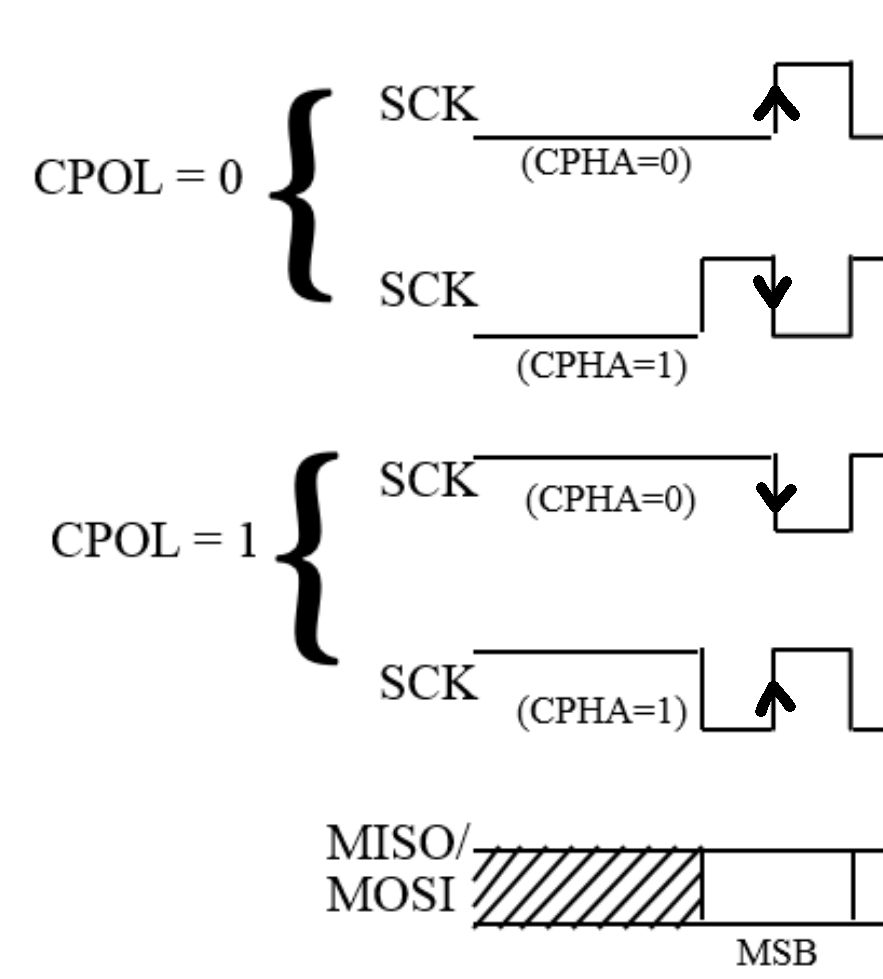
\includegraphics[width=.5\columnwidth]{"Images/SPI_Clock_modes.png"}
\end{center}

SPI can be setup in form of a Point-to-Point, Star or Ring topology.
There are implementations with multiple parallel datalines between master and slave (Dual-, Quad- Octal-SPI).


\subsection{I2C \refskript{9.4.2}}
See \refskript{Figure 9.25 and 9.26} for the message structure.
Max addresses: \formula{$2^{\text{\#-addr-bits}} - 16$} (Two 8-bit blocks are reserved).
For clock arbitration, see \refskript{Fig. 9.29}.

\begin{lstlisting}[language=C]
i2cError_t hal_i2c_dataRead(uint8_t slaveAddress, uint8_t* pData, uint8_t rxLen) {
	i2cError_t i2cError = I2C_NO_ERR;
	UCB1IFG = 0x0000;  // clear old flags
	
	// Set the address of the slave with which the master will communicate.
	UCB1I2CSA = slaveAddress;
	
	UCB1CTLW0 &= ~0x0010;  // receive mode
	UCB1CTLW0 |= 0x0002;   // generate start condition (start)
	while (UCB1CTLW0 & 0x0002);  // wait until start condition sent
	
	if ((UCB1IFG & 0x0020) == 0x00)  // check if no error occured
	{
		for (; rxLen > 1; rxLen--) {
			while (!(UCB1IFG & 0x0001)); // wait until receive is complete (RXIFG)
			*pData = UCB1RXBUF;  // get single byte data
			pData++;
		}
	} else {
		i2cError = I2C_ADDR_ACK_ERR;  // nack received --> no valid slave address
	}
	
	UCB1CTLW0 |= 0x0004;  // send as next the stop condition
	while (!(UCB1IFG & 0x0001)); // wait until receive is complete
	*pData = UCB1RXBUF;  // get last single byte data
	while (UCB1CTLW0 & 0x0004);  // wait until stop has complete sent
	return i2cError;
}
\end{lstlisting}
